You can debug Caesar programs using the normal Java debugger. To set a breakpoint, right-click in the gutter of the editor and choose "Toggle Breakpoint", or simply double-click in the gutter.\\\\
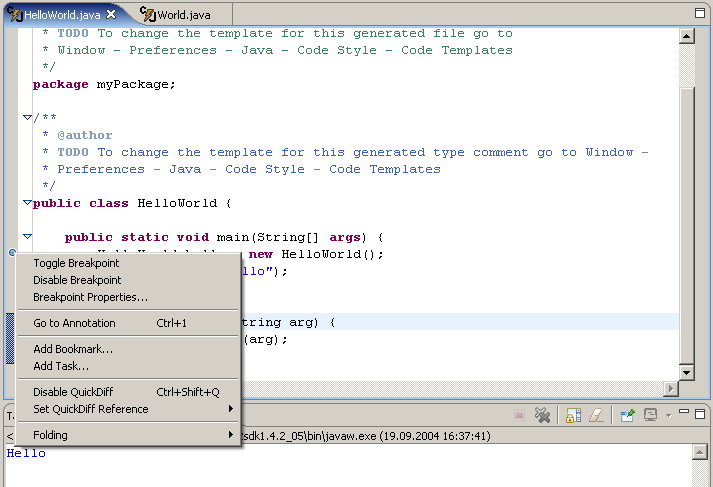
\includegraphics[width=0.90\textwidth]{images/brake_point.png}\\

With one or more breakpoints set, you launch the Eclipse debugger in the normal way by clicking on the debug icon in the toolbar.\\\\
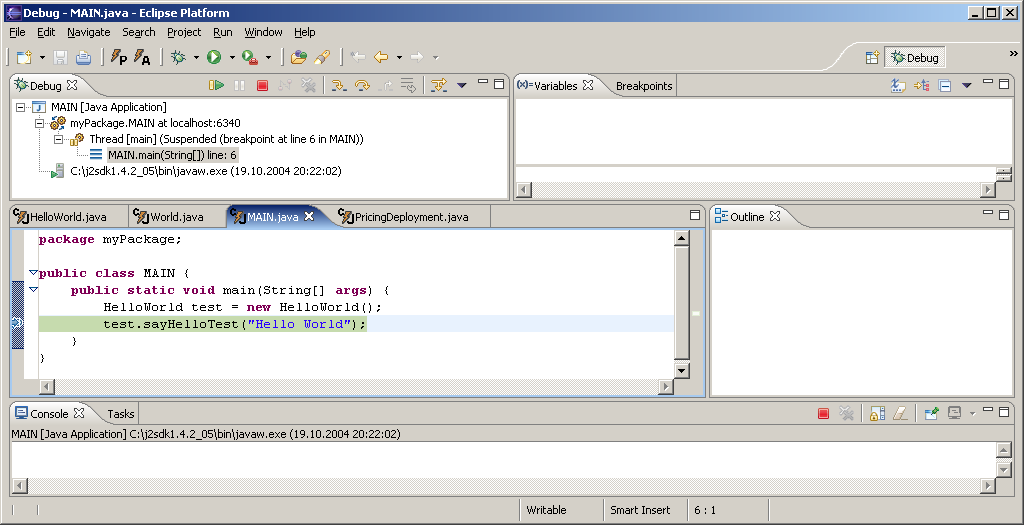
\includegraphics[width=0.80\textwidth]{images/debug1.png}\newpage

You can use the Java Debug step filters (Window -$>$ Preferences -$>$ Java -$>$ Debug -$>$ Step Filtering) to make this process a little easier.
Note: A current limitation is that you cannot step into advices.